

\section{What is the Earth System Modeling Framework?}

The Earth System Modeling Framework (ESMF) is a suite of software
tools for developing high-performance, multi-component Earth science
modeling applications.  Such applications may include a few or dozens
of components representing atmospheric, oceanic, terrestrial, or
other physical domains, and their constituent processes (dynamical, chemical,
biological, etc.).  Often these components are developed by different
groups independently, and must be ``coupled'' together using software
that transfers and transforms data among the components in order to form
functional simulations.

ESMF supports the development of these complex applications in a number
of ways.  It introduces a set of simple, consistent component interfaces
that apply to all types of components, including couplers themselves.  These
interfaces expose in an obvious way the inputs and outputs of each component.
It offers a variety of data structures for transferring data between components, 
and libraries for regridding, time advancement, and other common modeling
functions.  Finally, it provides a growing set of tools for using metadata
to describe components and their input and output fields.  This capability
is important because components that are self-describing
can be integrated more easily into automated workflows, model and dataset
distribution and analysis portals, and other emerging ``semantically enabled''
computational environments.

ESMF is not a single Earth system model into which all components
must fit, and its distribution doesn't contain any scientific code.
Rather it provides a way of structuring components so that they can be used 
in many different user-written applications and contexts with minimal code
modification, and so they can be coupled together in new configurations
with relative ease.  The idea is to create many components across a
broad community, and so to encourage new collaborations and combinations.

ESMF offers the flexibility needed by this diverse user base.  It is tested
nightly on more than two dozen platform/compiler combinations; can be
run on one processor or thousands; supports shared and distributed memory
programming models and a hybrid model; can run components
sequentially (on all the same processors) or concurrently (on mutually
exclusive processors); and supports single executable or multiple
executable modes.

ESMF's generality and breadth of function can make it daunting for the
novice user.  To help users navigate the software, we try to apply
consistent names and behavior throughout and to provide many examples.
The large-scale structure of the software is straightforward.
The utilities and data structures for building modeling components 
are called the ESMF {\it infrastructure}.  The coupling interfaces and
drivers are called the {\it superstructure}.  User code sits between
these two layers, making calls to the infrastructure
libraries underneath and being scheduled and synchronized by the 
superstructure above.  The configuration resembles a sandwich, as
shown in Figure~\ref{fig:TheESMFwich}.

ESMF users may choose to extensively rewrite their codes
to take advantage of the ESMF infrastructure, or they may decide to
simply wrap their components in the ESMF superstructure in order to
utilize framework coupling services.  Either way, we encourage users
to contact our 
\htmladdnormallink{support team}{mailto:esmf\_support@ucar.edu}
 if questions arise about how to best
use the software, or how to structure their application.  ESMF is
more than software;  it's a group of people dedicated to realizing
the vision of a collaborative model development community that spans
institutional and national bounds.



The Earth System Modeling Framework (ESMF) is a structured collection of 
software building blocks that can be used or customized to develop 
Earth system model components, and assemble them into applications.  
The simplest view of the ESMF is that it consists of an {\it infrastructure} 
of utilities and data structures for creating 
model components, and a {\it superstructure} for coupling them.  
User code sits between these two layers, making calls to the infrastructure
libraries beneath it and being scheduled and synchronized by the 
superstructure above it.  The configuration resembles a sandwich, as
shown in Figure~\ref{fig:TheESMFwich}.

The ESMF architecture is scalable, flexible paradigm for building highly 
complex climate, weather, and related applications from components such
as atmospheric models, land models, and data assimilation systems.  The 
ESMF is not a single master application into which all components must fit; 
rather it is a way of developing components so that they can be used 
in many different user-written applications.  Model components that adopt 
ESMF are designed to be usable in different contexts with minimal code
modification, and may be
incorporated into other ESMF-based modeling systems within the Earth 
science community.  In addition to high-level organization, ESMF provides 
a set of robust, portable, performance optimized libraries for regridding, 
data transfers, time management, and other common modeling functions.  
ESMF users may choose to extensively rewrite their codes to take advantage 
of the ESMF infrastructure, or they may decide to simply wrap user-written 
components in ESMF interfaces in order to adopt the ESMF architecture and 
utilize framework coupling services.

\section{The ESMF User's Guide}

This {\it ESMF User's Guide} is mainly an installation and build guide for
the new ESMF user and a build reference for the experienced user.  
New users are strongly encouraged to download the ESMF software and try
running a demonstration program, {\tt ESMF\_COUPLED\_FLOW}, that illustrates
both ESMF utilities and coupling services.  

The {\it User's Guide} is organized as follows.  The next two sections, 
\ref{sec:Support} and \ref{sec:Submission}, 
concern user support and how to submit comments on the ESMF system 
to our development team.  
Sections \ref{sec:QuickStart} through \ref{sec:TechOver2} contain a 
{\it Quick Start} guide that explains how to install the ESMF software 
and run the self-tests, 
followed by more detail on ESMF structure and operation, 
such as a description of the directory structure and how to build and
run the ESMF examples and demonstration programs.
Section \ref{sec:ArchOver} is an architectural overview that describes the
framework's basic goals and features.  The next few Sections, beginning
with \ref{sec:demo}, describe in detail the {\tt ESMF\_COUPLED\_FLOW} demo
application.
Section \ref{sec:Adoption} details the steps required to adapt a component
for use with ESMF.  Finally, to help you become familiar with ESMF
terminology, the last section in the {\it User's Guide} is a glossary.

\begin{center}
\begin{figure}
\caption{Schematic of the ESMF ``sandwich'' architecture. In this 
design the framework consists of two parts, an upper level
{\bf superstructure} layer and a lower-level {\bf infrastructure} layer. 
User code is sandwiched between these two layers.}
\label{fig:TheESMFwich}
\scalebox{1.0}{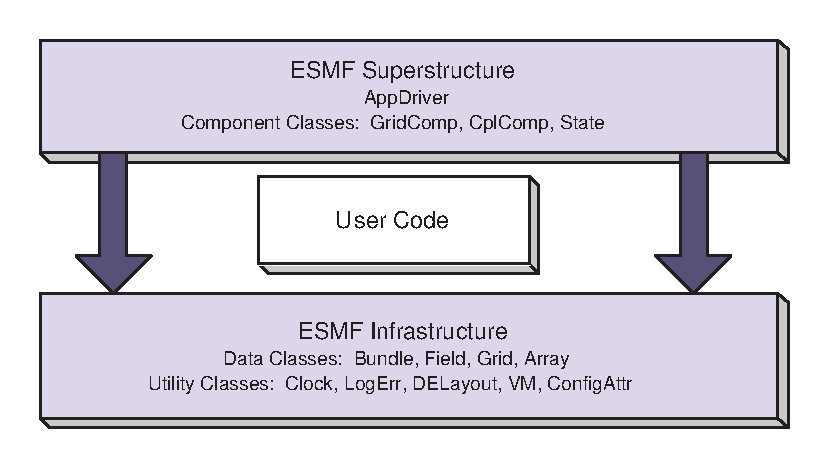
\includegraphics{ESMF_sandwich}}
\end{figure}
\end{center}


